\section{Softcore Nios II}		
	\subsection{Soft-Core vs. Hard-Core Processors \weekMaehne{2}}
		\begin{table}[H]
			%\centering
			\begin{tabular}{|p{0.7\linewidth}|p{0.25\linewidth}|}
				\hline
				\textbf{Soft-Core} 
				& \textbf{Hard-Core}\\
				\hhline{|=|=|}
				Synthesised by a logic compiler in HDL and placed and routed on the FPGA 
				& Fixed implementation in silicon\\
				\hline
				Can be modified according to requirements (more features, custom instructions etc.) 
				& No modifications possible\\
				\hline
				Speeds up to $250MHz$
				& Speeds up to $>1GHz$\\
				\hline			
			\end{tabular}
		\end{table}
	
	\subsection{The Nios II \weekMaehne{2}}
		\begin{multicols}{2}
			\begin{compactitem}
				\item 32 bit RISC Architecture
				\item 256 instructions available for user implementation
				\item Variants to fine-tune: speed / area / power
				\item Operating systems supported: Linux, embOS, RTOS
				\item Harward Architecture
				\item Little-Endian Byte Ordering
			\end{compactitem}
		\end{multicols}
	
	\subsection{Custom Components and Instructions \weekMaehne{2}} 
		\begin{minipage}[H]{0.8\textwidth}
			\begin{compactitem}
				\item Custom components and instructions can increase system performance
				\item Usually code-parts which are often executed by software are out-sourced into hardware
				\item Custom logic is integrated into the NIOS processors ALU
				\item Custom Instructions can take two values from up to two source registers and write back a result to a destination register
				\item Custom instructions appear as assembly macros or C functions
				\item Types of instructions:
					\begin{compactitem}
						\item Combinatorial Instructions
						\item Multi-cycle, synchronized by clk
						\item Parametrized
					\end{compactitem}
			\end{compactitem}
		\end{minipage}
		\begin{minipage}[H]{0.2\textwidth}
			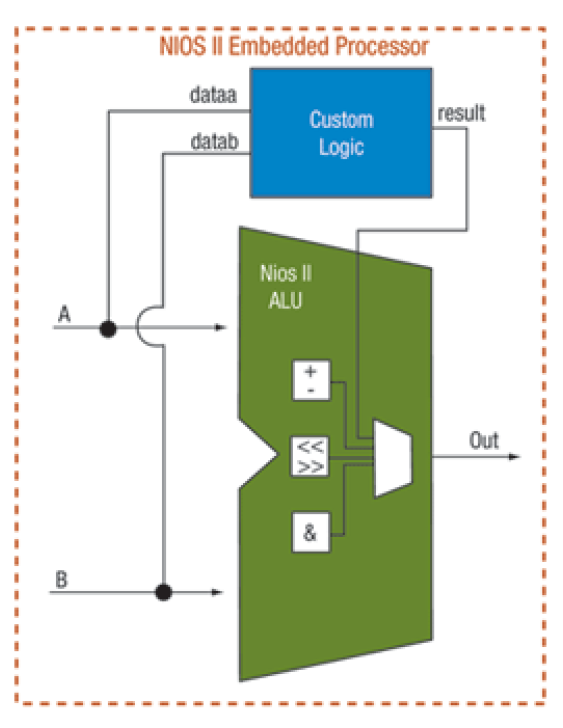
\includegraphics[width=0.9\textwidth]{./pictures/custom_instruction.png} 
		\end{minipage}
	
	\subsection{Interrupt Controller \weekPageMaehne{2}{10}}
		\begin{multicols}{2}
			\begin{compactitem}
				\item The Nios II supports 32 internal hardware interrupts				
				\item Each interrupt can be enabled separately via the \lstinline[style=C]{isenable} Register
				\item Priority is set by software
				\item Interrupts can be globally enabled with the \lstinline[style=C]{PIE} bit of the status register
			\end{compactitem}
		\end{multicols}
	
	\subsection{Memory Resources \weekMaehne{2}}
		The most important memory interfaces are:
		\begin{multicols}{2}
			\begin{compactitem}
				\item Instruction master port: Avalon-MM master port that connects to instruction memory
				\item Instruction cache (Internal)
				\item Tightly-coupled instruction or data memory port
				\item Data master port: Avalon-MM master port that connects to data memory and peripherals
				\item Data cache (Internal)				
			\end{compactitem}
		\end{multicols}
	
		\subsubsection{Tightly coupled Memory \weekPageMaehne{2}{14}}
			\begin{multicols}{2}
				\begin{compactitem}
					\item Performance is similar to cache memory.
					\item Software can guarantee that performance-critical code or data is located in tightly-coupled memory.
					\item No real-time caching overhead, such as loading, invalidating, or flushing memory.
					\item An On-Chip Memory component is the only memory that can be used.
					\item Each tightly-coupled memory is directly connected to a master port.
				\end{compactitem}
			\end{multicols}